\documentclass[10pt,a4paper]{article}
\usepackage[ngerman]{babel}
\usepackage[utf8]{inputenc}
\usepackage{graphicx}
\usepackage{titling}
\bibliographystyle{alpha}
\usepackage[left=2.5cm,right=2.5cm]{geometry}
\usepackage{floatrow}
\usepackage{wrapfig}


%PDF Hyperlinks
\usepackage{hyperref}
\hypersetup{pdftex}
\usepackage{hypcap}

\usepackage{color}
\definecolor{green}{rgb}{0.0, 0.65, 0.31}
\usepackage{listings} 
\lstset{
	numbers=left, 
	numbersep=12pt,
	commentstyle=\color{green},
	basicstyle=\small
} 
\usepackage{hyperref}
\lstset{language=Matlab} 


% Add subtitle-command
\newcommand{\subtitle}[1]{%
  \posttitle{%
    \par\end{center}
    \begin{center}\large#1\end{center}
    \vskip0.5em}%
}

\begin{document}
\begin{titlepage}
\vspace*{1cm}
\begin{center}
\Huge
Technische Hochschule Nürnberg\\
\vspace*{2cm}
\large
 {\Large Projektarbeit im Wahlpflichtfach Softcomputig\\
Dozent: Prof. Dr. Reinhard Eck\\}
\vspace*{2cm}
\Huge
Neuronale Netze\\
\large
\vspace*{1cm}
Praktische Anwendung bei der automatischen Erkennung von Captchas
\vspace{1cm}

\vspace{2cm}

 \begin{tabular}{p{6 cm}p{6 cm}}
    	vorgelegt von & {Christopher Althaus} \\
		& {Baris Akdag} \\
		& {Matthias Jentsch} \\
		\\ & \\
    	Abgabe:& 1. Juli 2013
 \end{tabular}\\
    


\end{center}
\end{titlepage}

\tableofcontents

% Hier bitte alle selbst geschriebenen Kapiel einfügen. 
\include{Fachartikel}
% Motivation, Einsatz im täglichem Leben...,  						//Baris
% Captcha Generator 												//Baris

% Lösungsansatz, Grober Programm Ablauf, Aufbau des Neuronalen Netzes //Matze
\section{Konzept}

Diese Sektion enthält eine Beschreibung des generellen Lösungsansatzes, der in
den einzelnen Phasen des Programmes verfolgt wird. Eine detaillierte Dokumentation
der konkreten Umsetzung befindet sich in Sektion \ref{module} - Modulbeschreibung.

Um eine hohe Erkennungsrate der Captchas zu erreichen und den Rechenaufwand
gering zu halten, haben wir uns dazu entschieden
uns nicht ausschließlich auf die Funktion des neuronalen Netzes zu verlassen
und stattdessen im Programmablauf Vorbereitungsphasen zu integrieren, die die
Daten für das neuronale Netz aufbereiten. Durch diese Aufbereitung wollen wir
die Zahl der Inputneuronen gering halten und eventuelle Störsignale bereits Image
Voraus entfernen.

Aufgrund dieser Anforderungen haben wir uns bei der Umsetzung für Matlab entschieden, 
da es bereits passende Erweiterungen zur Aufbereitung von Bildern und zum
Erstellen von neuronalen Netzen speziell für die Mustererkennung bietet.


\subsection{Ablaufphasen des Programms}

Der Ablauf des Programms kann in folgende grobe Phasen unterteilt werden: 

\begin{itemize}

\item Trainingsphase

Erstellen des neuronalen Netzes.


\item Einlesen und Aufbereiten der Captchas

Liest die Captchas aus den Dateien ein und entfernt grobe Störsignale.


\item Segmentierung

Teilt die aufbereiteten Bilder in einzelne Zeichen und normalisiert die
Ausrichtung.


\item Datenaggregation

Zusammenfassen von verwandten Datensätzen um die Anzahl der Eingaben zu reduzieren.


\item Klassifizierung

Erkennen der Zeichen durch das neuronale Netz

\end{itemize}


\subsubsection{Trainingsphase}

Die Trainingsphase ist die Phase in der ein neuronales Netz zum Erkennen der
Zeichen erstellt wird. Die Trainingsphase soll nur dann aufgerufen werden, wenn
nicht bereits ein Vorbereitetes Netz existiert. In der Trainingsphase werden
vorbereitete Captchas zusammen mit der Lösung eingelesen und analog zu den
normalen Bildern aufbereitet. Die einzelnen Zeichen werden zusammen mit dem
Ergebnis zum Trainieren des Neuronalen Netzes verwendet. Die Trainingsphase
soll so lange andauern, bis sich zwischen den einzelnen Trainingsphasen keine
relevante Verbesserung ergibt.

\subsubsection{Einlesen und Aufbereiten der Captchas}

\begin{wrapfigure}[6]{r}{5cm}
  \begin{center}
  \vspace{-48pt}
    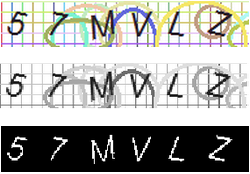
\includegraphics[width=4cm]{res/Aufbereitung.png}
  \end{center}
  \caption{Aufbereitung eines Captchas}
\end{wrapfigure}

In diesem Schritt werden alle Bilder aus einem Eingabeverzeichnis eingelesen und
aufbereitet. Die Aufbereitung versucht alle Pixel, die nicht zum eigentlichen
Text gehören herauszufiltern. Zudem werden Farben durch binäre Werte ersetzt
die entweder Schwarz oder Weiß darstellen. Hierbei wird anhand eines
Schwellwertes unterschieden ab wann ein Graustufenwert als Schwarz oder als
Weiß gilt. Eine genauere Beschreibung der Aufarbeitung der Bilder befindet sich
in Kapitel \ref{images} - Aufbereitung von Bildern mit der Matlab-Image-Toolbox.


\subsubsection{Segmentierung}
\label{segment}

  \begin{wrapfigure}[6]{R}[0pt]{6cm}
  \vspace{-35pt}
  \begin{center}
    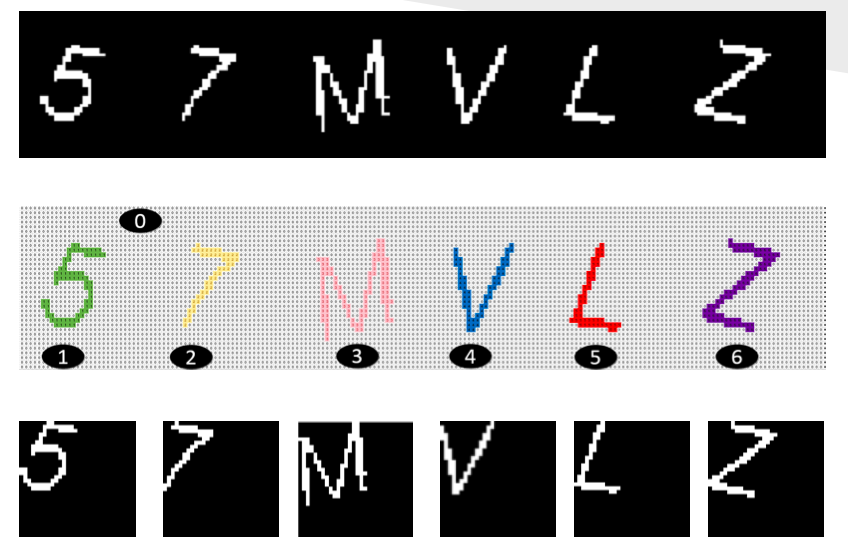
\includegraphics[width=5cm]{res/Segmentierung.png}
  \end{center}
  \vspace{-5pt}
  \caption{Segmentierung}
  \vspace{-10pt}
\end{wrapfigure}


Bei der Segmentierung wird versucht die Zeichen des Worts in einzelne Segmente
zu unterteilen. Da das neuronale Netz eine konstante Menge an Eingabewerten
benötigt, wird zudem die Auflösung der Segmente auf eine Einheitliche größe
Festgelegt. Alle Zeichen werden auf die gleiche Art ausgerichtet um
Verschiebungen auszugleichen.

\subsubsection{Datenaggregation}

\begin{wrapfigure}[15]{R}[0pt]{7cm}
  \begin{center}
    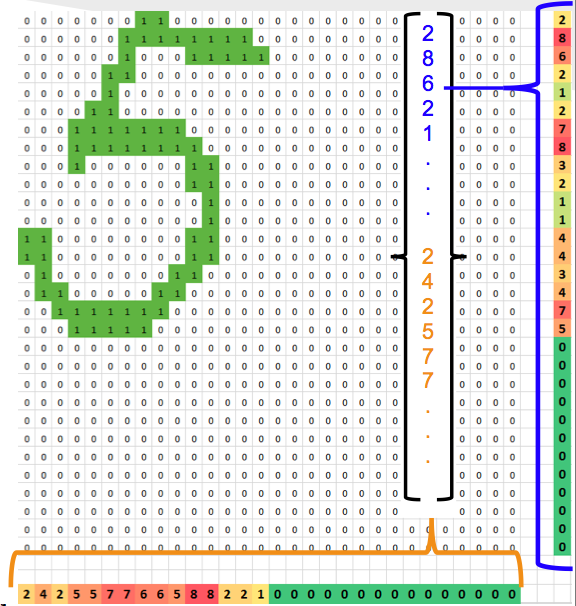
\includegraphics[width=6cm]{res/Aggregation.png}
  \end{center}
  \vspace{-5pt}
  \caption{Aggregation der Spalten/Zeilen}
  \vspace{-10pt}
\end{wrapfigure}


Bei der Datenaggregation wird versucht die Menge an Eingabewerten zu reduzieren,
ohne dabei viel Genauigkeit zu verlieren. Dies wird erreicht indem 
die Summen aller Schwarzen Pixel pro Zeile und Spalte gebildet wird. 

Ohne diese Aggregation, also bei direkter Eingabe aller Pixel in das
neuronale Netz, wäre die Laufzeit des Lernvorgangs und der Mustererkennung zu
hoch um das Programm sinnvoll verwenden zu können.
\subsubsection{Klassifizierung}

Die Klassifizierung benutzt das neuronale Netz, um die eigentliche
Mustererkennung durchzuführen und so die einzelnen Buchstaben zu
erkennen. Jede Summe aus der Datenaggregation wird als einzelner Eingabewert
für das Netz verwendet. Diese Werte sollen in Matlab in Form eines Vektors zu
einem Set aus Eingabewerten für ein einzelnes Zeichen zusammengefasst werden.

\section{Struktur des neuronalen Netzes}

Um festzustellen wie viele Hidden-Neuronen das Netz braucht, wurde die
Leistungsfähigkeit des Netzes bei verschiedensten Mengen an Neuronen getestet.
Um die Leistungsfähigkeit der Netze auszuwerten wurde die Zahl der richtig
erkannten Captchas ausgewertet. 

Für jede Messung wurde automatisiert ein neues Neuronales Netz mit der aktuellen
Anzahl der Hidden-Neuronen erstellt und dessen Leistungsfähigkeit gemessen.
Die Ergebnisse der Messung sind in folgender Grafik dargestellt:

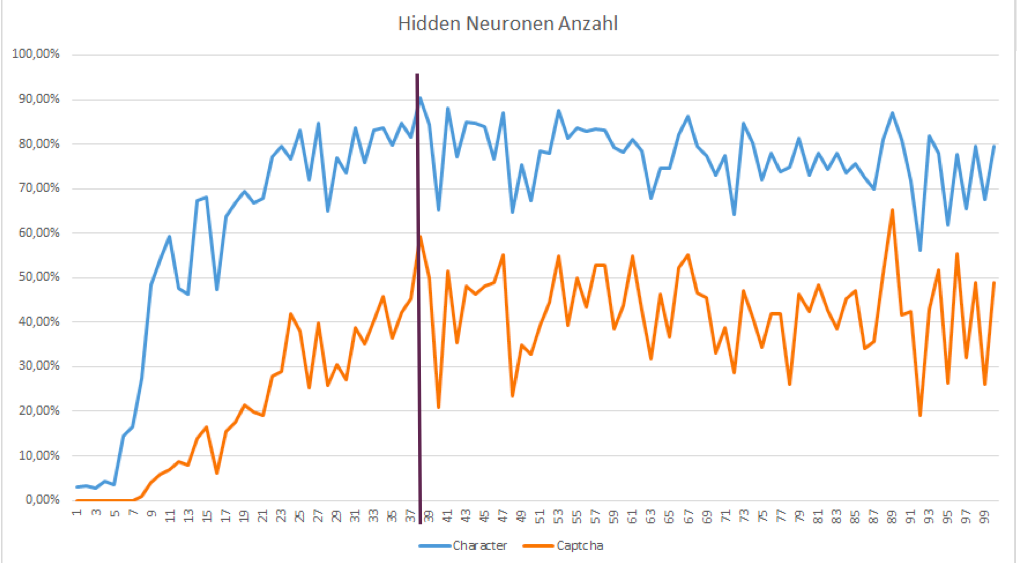
\includegraphics[width=14cm]{res/performance.png}

Da der Anstieg der Leistungsfähigkeit ab etwa $38$ Hidden-Neuronen aufhört,
legen wir die Anzahl dieser auf $38$ fest.

\subsection{Matlab - Die Klasse ``Patternnet''}

In der Matlab-Toolbox für neuronale Netze existiert bereits ein vorgefertigtes
neuronales Netz für die Mustererkennung. Diese Klasse nennt sich ``Patternnet''
und erbt von der Basisklasse ``nnet''. Die Klasse erstellt ein Feedforward-Netz
mit der Lernfunktion ``trainscg'', die die Konjugierte Gradientenmethode zum
Lösen der Gleichungssysteme, die die neuen Gewichtungen bestimmen, verwendet.


  \begin{center}
    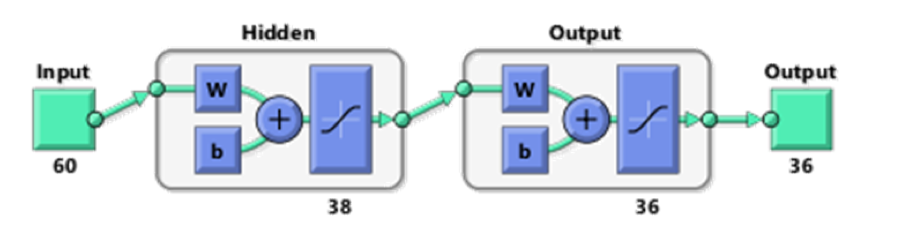
\includegraphics[width=12cm]{res/PatternNet-Aufbau.png}
  \end{center}


\subsection{Transferfunktion}
 Als Transferfunktion wird ein Sigmoid mit der folgenden Gleichung verwendet:

\begin{wrapfigure}[10]{R}[0pt]{7cm}
  \begin{center}
    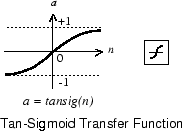
\includegraphics[width=6cm]{res/tansig.png}
  \end{center}
\end{wrapfigure}

\begin{equation}
n = tansig(n) =  \frac{2}{(1 + e^{-2*n})} - 1
\end{equation}

Der Wert von $n$ berechnet sich aus den aufsummierten, gewichteten
Eingsangswerten:

\begin{equation}
  n = w_1 * i_1 + w_2 * i_2 + \ldots  + w_j * i_j
\end{equation}

Das Sigmoid bewirkt, dass sich die Ausgabewerte eines Neurons ausschließlich
im Bereich $[-1,1]$ befinden. Zudem ist die Funktion einfach ableitbar, was
hilfreich beim aktualisieren der Gewichtungen während des Lernvorgangs ist.

\subsubsection{Lernfunktion}

In jeder Runde des Lernvorgangs müssen die Gewichte des Netzes so verändert werden,
dass sie möglichst nah am gewünschten Ausgangswert sind. Hierfür ist es
notwendig ein Gleichungssystem zu lösen um den optimalen Wert zu finden. Die Lernfunktion
des ``Patternnet'' verwendet hierfür die Konjugierte Gradientenmethode, die ein
numerisches, iteratives Verfahren zum Lösen des Gleichungssystems darstellt.


\section{Aufbereitung von Bildern mit der Matlab-Image-Toolbox}
\label{images}

Für die Aufbereitung der Captchas werden Funktionen aus der Matlab
Image-Toolbox verwendet. Die wichtigste ist hierbei die Funktion $regionprops$,
die dazu in der Lage ist, auf einem Bild Regionen mit bestimmten Eigenschaften
zu markieren. So ist es beispielsweise möglich, Regionen die sich in ihren Farb-
werten nicht stärker als ein bestimmter Grenzwert unterscheiden, zu markieren.
Mithilfe dieser Technik werden auf dem Captcha zusammenhängende Buchstaben 
gefunden. Bei der Segmentierung, die in Sektion \ref{segment} beschrieben wird,
ist es essenziell diese Regionen zu kennen um zu vermeiden, dass die Zeichen an
der falschen Stelle zerteilt werden.

% \subsection{Darstellung von Bildern in Matlab}
% Bilder werden in Matlab generell wie Matritzen behandelt. Je nach Farbtiefe der
% Bilderm enthält jeder Wert entweder einen RGB- oder Graustufenwert. 


% Bild aufbearbeitung (Toolbox image)								// Matze
\include{bildaufbereitung}
% Segmentierung Klassifizierung 									// Christopher

% Anleitung zur Benutzung 											// Christopher
\newpage
\section{Bedienungsanleitung}
\subsection{Voraussetzungen}
Um zu gewährleisten, dass die Matlab Module, dieses Projekts ordnungsgemäß funktionieren, wird eine Matlab Version R2013a oder höher mit folgenden Toolboxen benötigt:
\begin{itemize}
\item Neural Network Toolbox
\item Image Processing Toolbox
\end{itemize}
Für die Ausführung des Captcha Generators wird lediglich das .Net Framework 2.0 benötigt.

\subsection{Ordnerstruktur}
Da die Matlab Module auf eine fest definierte Ordnerstruktur zugreifen, ist es wichtig diese einzuhalten. Die Ordnerstruktur sollte der folgenden entsprechen.
\begin{verbatim}
Matlab/
  images/
    Test/
      Capture1.png
      Capture2.png
      ...
    Training/
      0ZEHSQ.png
      TWU7P8.png
      ...
  src/
    buildNetwork.m
    classify.m
    preprocess.m
    recognize.m
    runTest.m
    segment.m
\end{verbatim}
Wichtig ist, dass die Ordner, in welchen sich die Captcha befinden einmal zum Matlab Pfad hinzugefügt wurden. Dies kann mit Hilfe des Matlab Datei Explorers getan werden:
\begin{verbatim}
Rechtsklick auf den Ordner 'images'
  -> Add to Path
    -> Selected Folders and Subfolders
\end{verbatim}
Wenn die Ordner zum Pfad hinzugefügt wurden, sollten diese grau hinterlegt dargestellt werden. Weiterhin ist zu beachten, dass man sich während der Ausführung der Module stets im Ordner '/src' befinden muss. Dies ist erst der Fall, wenn in der Pfadangabe des aktuellen Ordners von Matlab '/src' steht!
\subsection{Generator}
Sollen neue Captcha generiert werden, kann beim Generator unter Target der Zielordner angegeben werden, in welchen die Captcha gespeichert werden sollen. Unter Files legt die Anzahl der zu erzeugenen Captcha fest und Chars die Anzahl der Zeichen pro Captcha. Es gilt zu beachten, dass die Matlab Module auf sechs Zeichen pro Captcha programmiert wurden, und es deshalb ohne entsprechende Codeanpassungen zu Fehlern kommt, sollten mehr oder weniger Zeichen in einem Captcha enthalten sein.\\
Mittels Angle lässt sich der Wertebereich des Neigungswinkels der Zeichen im Captcha eingrenzen.\\
Die Generierung der Captcha wird mittels des Start Button gestartet. Sobald die Captcha generiert wurden, erscheint eine Messagebox, die die erfolgreiche Erstellung bestätigt.

\subsection{Captcha Erkennung}
Die Erkennung von Captchas erfolgt ausschließlich in Matlab. Für eine erfolgreiche Erkennung ist es wichtig, das der Ordner, in welchem sich das Bild befindet, zum Matlab Pfad hinzugefügt wurde. Wie dies funktioniert, wird unter dem Punkt Ordnerstruktur erklärt.\\
Vor der Ausführung muss sich Matlab im Verzeichnis 'src' der Ordnerstruktur befinden. Die Abfrage eines einzelnen Captchas erfolgt mittels des 'recognize' Moduls, welches als Parameter den Namen der Bilddatei erwartet. Der Abruf erfolgt durch das Kommandofenster innerhalb von Matlab wie folgt:
\begin{verbatim}
>> recognize('ZVEEIO.png')

ans =

ZVEEIO
\end{verbatim} 
Wird die Anfrage nicht mit einem Semikolon abgeschlossen, gibt Matlab das Ergebnis direkt im Kommandofenster aus. Alternativ ist es auch möglich das Ergebnis der Abfrage einer Variable zuzuweisen:
\begin{verbatim}
>> capture = recognize('capture.png');
>> capture

capture =

ZVEEIO
\end{verbatim} 
$\;$ \\
Sollen mehrere Captcha gelöst werden, so können diese in den Ordner '/Test' der Ordnerstruktur gespeichert werden. Durch den Aufruf des Moduls 'runTest', werden automatisch alle Captcha durchlaufen, und die Ergebnisse direkt im Kommandofenster ausgegeben:
\begin{verbatim}
>> runTest();
1	 Aktuell: 0E0HSQ	 Erkannt: 0E0HSQ	 OK
2	 Aktuell: 0JDDQ2	 Erkannt: 0JDDQ2	 OK
3	 Aktuell: 0K42MH	 Erkannt: 0K42MH	 OK
4	 Aktuell: 1VVYE7	 Erkannt: 1VVYE7	 OK
5	 Aktuell: 1XHLLA	 Erkannt: 1XHLLA	 OK
\end{verbatim} 
% Fazit 															// Baris + Überarbeitung 

%Codedokumentation													//Christopher
\newpage
\section{Modulbeschreibung}
\label{module}
Zur Umsetzung des Projektes wurde verschiedene Module implementiert, welche im Folgenden der Reihe nach näher beschrieben werden sollen.
\subsection{Preprocessor}
Der Preprocessor bereinigt das ihm übergebene Captcha um die Artefakte.
\begin{lstlisting}
function cleaned = preprocess(image)

	greyScale = rgb2gray(image);
	cleaned = greyScale < 65;

end
\end{lstlisting}
Das Modul nimmt als einzigen Parameter ein Captcha als Bild entgegen und gibt als Rückgabewert das von Artefakten bereinigte Bild zurück. Da in diesem Projekt die neuronalen Netze im Vordergrund standen, ist die Bereinigung des Bildes denkbar einfach. Die vom Generator erzeugten Artefakte haben stets einen Grauwert, welcher über 65 liegt. Deshalb wird zunächst die Matlab Funktion \textit{rgb2gray} auf das übergebene Bild angewendet, welche das Bild in Graustufen umwandelt.\\
Anschließend werden in der Matrix \textit{cleaned}, die Bildpunkte, deren Grauwert kleiner 65 ist, auf eins gesetzt und alle anderen auf null.
\newpage
\subsection{Segmentierung}
Dieses Modul segmentiert das übergebene Bild in die einzelnen Buchstaben.
\begin{lstlisting}
function [retVal] = segment(bounded)

    retVal = zeros(30, 30, 6);

    cc = bwconncomp(bounded);
    labeled = labelmatrix(cc);
  
    charIndex = 1;
    while (charIndex <= 6)

        % Sucht die Position der einzelnen Pixel mit der gegebenen Buchstabenposition
        [yPx,xPx] = find(labeled == charIndex);
        singleChar = zeros(size(bounded)); 

        % Fuegt die Pixel des einzelnen Buchstaben in die leere Matrix ein
        singleChar(labeled == charIndex)= bounded(labeled == charIndex); 

        % Schneidet das einzelne Zeichen aus dem Gesamtbild heraus
        a = imcrop(singleChar, [min(xPx),  min(yPx),  max(xPx) - min(xPx), max(yPx) -  min(yPx)]);
        [charRows, charCols] = size(a);

        % Aendert die Matrixgroesse auf 30x30
        a = padarray(a, [(30 - charRows) (30 - charCols)], 'post');
        
        % Speichert das Bild in den Returnwert
        retVal(:,:,charIndex) = a;
        charIndex = charIndex + 1;
    end
end
\end{lstlisting}
Die Segmentierungs-Funktion erhält als Parameter das aufgearbeitete Bild des Preprocessors und gibt als Rückgabewert sechs Matrizen (es existieren stets sechs Zeichen pro Captcha) der Größe 30x30 als dreidimensionales Array zurück.\\
Zunächst wird in Zeile drei der Rückgabewert angelegt und die Matizen mit null initialisiert.\\
Zum eigentlichen Segmentieren der Zeichen aus dem Bild werden die Matlab Funktionen \textit{bwconncomp} und \textit{labelmatrix} verwenden, wobei \textit{bwconncomp} zusammenhängende Teile im Bild findet und \textit{labelmatrix} diese beginnend bei eins durchnummeriert. Das heißt, dass in der Matrix \textit{labeled} jedes der sechs im Captcha enthaltenen Zeichen nach Ausführung der sechsten Zeile durch eine bestimmte Zahl dargestellt wird. Die Pixel des ersten Zeichens wären also ''1'', die Pixel des zweiten Zeichens ''2'', usw.\\
Nachfolgend werden die einzelnen Zeichen der Reihe nach in die Variable \textit{retVal} abgespeichert. Dazu wird in einer while-Schleife jedes einzelne Zeichen aus dem Gesamtbild extrahiert (Zeilen 11-19) und anschließend in eine 30x30 große Matrix eingefügt (Zeile 23). 
\newpage
\subsection{Klassifizierung}
Das Klassifizierungsmodul berechnet den Input aus den übergebenen segmentierten Zeichen eines Captchas und ruft damit das neuronale Netz auf, welches für den Input eine Korrelation für die 36 Outputs erstellt.
\begin{lstlisting}
function decoded = classify(chars)
    load neuronal;
    decoded = char(zeros(1,6));
    
    for i=1:6
        inVP = sum(chars(:,:,i),2);
        inHP = sum(chars(:,:,i)',2);
        res = net([inVP;inHP]);
   
        % Sucht den Rueckgabewert mit der besten Korrelation
        index = find(res == max(res), 1);
        
        % Konvertiert das Rueckgabe-Ergebnis zurueck zu einem ASCII Zeichen
        if (index <= 10)
            index = index + 47;
        elseif (index >= 11 && index <= 36)
            index = index + 54;
        end

        decoded(i) = char(index);
    end
end
\end{lstlisting}
Zunächst wird in Zeile zwei das gespeicherte neuronale Netz geöffnet. Dieses gespeicherte Netz enthält die Variable \textit{net}, mit welcher später auf das Netz zugegriffen werden kann. In Zeile drei wird die Rückgabe in Form eines char-Feldes mit der Größe von sechs Feldern erzeugt.\\
Anschließend wird in den Zeilen sechs und sieben die Anzahl der vertikalen und horizontalen Pixel eines Zeichens gezählt. Dabei entsteht jeweils eine Matrix mit 30 Einträgen. Diese Matrizen werden aneinandergehängt und sind der Input für das neuronale Netz.\\
Die Variable \textit{res} beinhaltet nach der Ausführung von Zeile acht eine Korrelation für die 36 möglichen Zeichen. Das Zeichen, dessen Korrelation am höchsten ist, wird ausgewählt und anschließend zurück zu einem ASCII Zeichen konvertiert (Zeilen 11 - 18). Zum Schluss wird das konvertierte Zeichen an der richtigen Position in der Variable \textit{decoded} gespeichert, welche nach der Ausführung zurückgegeben wird. 

\newpage
\subsection{Generator}
Das \textit{buildNetwork}-Modul generiert das neuronale Netz aus den Captcha Bildern, die im Trainingsordner abgespeichert sind.
\begin{lstlisting}
function [net, training] = buildNetwork()

    trainingDir = '../images/Training/';
    trainingSamples = dir(strcat(trainingDir, '*.png'));
    [numTrainingSamples] = size(trainingSamples);
    trainingSamplesSize = numTrainingSamples(1,1) * 6;
    in = zeros(60,trainingSamplesSize);
    out = zeros(36,trainingSamplesSize);
    
    % Erstellt ein Pattern Recognition Netzwerk
    net = patternnet(38);
    net.divideParam.valRatio = 0;
    net.divideFcn = 'dividerand';
    net.divideMode = 'sample';
    net.divideParam.trainRatio = 70/100;
    net.divideParam.valRatio = 15/100;
    net.divideParam.testRatio = 15/100;
    net.trainParam.goal = 0.0001;
    net.performFcn='msereg'; 
  
    for i=1:numTrainingSamples
        filename = strcat(trainingDir, trainingSamples(i).name);  
        bounded = preprocess(imread(filename));     
        chars = segment(bounded);
        % Ordnerpfad von Dateinamen entfernen
        filename = strrep(filename, trainingDir, '');
        for j=1:6
            % Konvertiert von ASCII zu int 
            % Zahlen liegen nachher im Bereich 1 - 10
            % Buchstaben liegen im Bereich 11 - 36
            asciiz = uint8(filename(j));
            if (asciiz >= 48 && asciiz <= 57)
                asciiz = asciiz - 47;
            elseif (asciiz >= 65 && asciiz <= 90)
                asciiz = asciiz - 54;
            end
            % Summiert die Anzahl der Horizontalen und Vertikalen Pixel
            inVP = sum(chars(:,:,j),2);
            inHP = sum(chars(:,:,j)',2);
            % Speichert die berechneten Matizen in den Input des Neuronalen
            % Netzes und den Buchstabenwert in den Output
            in(:,(i-1)*6+j) = [inVP;inHP];
            out(asciiz,(i-1)*6+j) = 1;
        end
    end
    % Trainiert das Netzwerk
    [net, training] = train(net,in,out);       
end
\end{lstlisting}
Die Generierungsfunktion erwartet keine Parameter beim Aufruf und gibt als Rückgabewert das generierte neuronale Netz und dessen Trainingsdaten zurück.\\
Damit ein Netz generiert werden kann, müssen im Ordnerpfad ''../images/Training/'' Captchas gespeichert sein, deren Dateiname dem Inhalt des jeweiligen Captchas entspricht.\\
Zunächst werden zwei Matrizen (\textit{in} und \textit{out}) erzeugt, in die für alle Captchas die zugehörigen Outputs zu den jeweiligen Inputs gespeichert werden.\\
Das neuronale Netz wird in den Zeilen 11 bis 19 initialisiert. Dabei wird die Anzahl der Inputs(60), Outputs(36) und der Hidden-Neuronen(38) festgelegt. Zudem werden weitere Feinabstimmungen des Netzes vorgenommen.\\
Innerhalb der for-Schleife werden auf die einzelnen Captchas der Reihe nach erst der Preprocessor und dann die Segmentierung angewendet. Anschließend wird der Input und der Output für jedes Zeichen eines Captchas erzeugt. Dabei wird für den Input, wie bei der Klassifizierung auch, die Summe der horizontalen und vertikalen Pixel genutzt (Zeilen 38-42). Für den Output wird aus dem Dateinamen an der jeweiligen Position im Captcha das entsprechende Zeichen gesucht und daraufhin dessen Position innerhalb der Output Matrix auf eins gesetzt (Zeilen 31-35 und Zeile 43). Zum Schluss wird das Netzwerk mittels der Funktion \textit{train} trainiert, welche als Parameter das initialisierte Netz und die berechneten In- und Outputs bekommt. Als Rückgabe resultiert das generierte Netz und dessen Trainingsdaten.

\newpage
\subsection{Erkennung}
Das Erkennungs-Modul führt die Funktionen, die für die Captcha-Erkennung nötig sind, aus und liefert die erkannten Zeichen als Ergebnis zurück.
\begin{lstlisting}
function decoded = recognize(imageFileName)
    % Prueft ob das Neuronale Netz existiert
     if (exist('neuronal.mat', 'file') == 0)
        fprintf('Neuronales Netz existiert nicht und wird jetzt generiert ...\n');
        trainPerf = 1;
        trainCount = 0;
        while(trainPerf > 0.002 && trainCount < 5)
            fprintf('%d. Generierung wird gestartet ...\n', trainCount+1);
            [net, training] = buildNetwork();
            if(trainPerf > training.best_perf)
                trainPerf = training.best_perf;
                save('neuronal.mat', 'net');
            end
            trainCount = trainCount + 1;
        end
    
        fprintf('Fertig (Trainingsperformance: %f)\n', trainPerf);
    end
    % 1. Laedt das Bild und fuehrt das Preprocessing durch
    preprocessed = preprocess(imread(imageFileName));
    
    % 2. Segmentiert das Bild
    segmented = segment(preprocessed);
    
    % 3. Decodiert die Buchstaben
    decoded = classify(segmented);
end
\end{lstlisting}
Die Funktion erwartet als Parameter den Dateinamen eines Captchas und gibt ein char-Feld mit den erkannten Zeichen zurück.\\
Im Vorab wird überprüft, ob das neuronale Netz bereits existiert. Ist dies nicht der Fall, wird die Generierung des Netzes angestoßen(Zeile neun). Um ein möglichst gutes neuronales Netz zu erhalten, wird die Trainingsperformance ausgewertet. Liegt die mittlere quadratische Fehlerabweichung über 0,002 wird eine erneute Generierung angestoßen. Maximal werden fünf Generierungen durchgeführt. Sollte auch dann die Trainingsperformance noch nicht unter 0.002 liegen, wird dass bis dahin am besten generierte Netz benutzt.\\
Ist das neuronale Netz generiert, werden der Reihe nach die Funktionen des Preprozessors, der Segmentierung und der Klassifizierung aufgerufen, wobei die Klassifizierung das Ergebnis zurückliefert, welches auch als Rückgabe an den Aufrufer der Erkennungs-Funktion zurückgegeben wird.
\newpage
\subsection{Testlauf}
Das Modul \textit{runTest} dient hauptsächlich dem Testen des neuronalen Netzes. 
\begin{lstlisting}
function[charAcc, capAcc] = runTest()
    testingDir = '../images/Test/';    
    testingSamples = dir(strcat(testingDir, '*.png'));
    numTestingSamples = size(testingSamples, 1);
    charCorrect = 0;
    charWrong = 0;
    captureWrong = 0;
    for i=1:numTestingSamples
        filename =  testingSamples(i).name;
        % Ruft die Recognize Funktion auf und bekommt die erkannten Zeichen zurueck
        chars = recognize(strcat(testingDir,filename));
        filename = strrep(filename, '.png', '');
        fprintf('%d\t Aktuell: %s\t Erkannt: %s\t', i, filename, chars);
        % Prueft komplettes Captcha auf Uebereinstimmung
        if (strcmp(filename, chars) == 0)
           fprintf(' NOK\n');
           captureWrong = captureWrong + 1;
        else
           fprintf(' OK\n');
        end
        % Prueft die einzelnen Zeichen auf Uebereinstimmung
        for j=1:6
          if (strcmp(filename(j), chars(j)) == 0) 
              charWrong = charWrong + 1;
          else
              charCorrect = charCorrect + 1;
          end
        end   
     end
     charAcc = charCorrect / (charCorrect + charWrong);
     capAcc = (numTestingSamples - captureWrong) / numTestingSamples;
     fprintf('Buchstaben Erkennungsrate: %f\n', charAcc);
     fprintf('Captcha Erkennungsrate: %f\n', capAcc);
end
\end{lstlisting}
Das Modul dient dem einfachen Auswerten der Erkennungsrate des neuronalen Netzes. Es erwartet keine Parameter und gibt die Erkennungsrate der einzelnen Zeichen eines Captchas und die Erkennungsrate der gesamten Captchas aus dem Test-Verzeichnis zurück.\\
Das Modul durchläuft in einer for-Schleife alle Test-Captchas die sich im Verzeichnis ''../images/Test'' befinden und ruft für diese die Erkennungs-Methode auf (\textit{recognize} Zeile 12). Anschließend werden die vom neuronalen Netz erkannten Zeichen mit den tatsächlich richtigen aus dem Dateinamen verglichen (Zeilen 15-28). Sind alle Captchas durchlaufen, wird die Gesamtfehlerquote pro Zeichen und pro Captcha ausgegeben.

\nocite{*}
\bibliography{Quellen.bib}

\end{document}
